\section{Methodology}

\subsection{TimeART}
\label{sec: timeart}
We make ReAct-style definitions of agentic time series reasoning for clear clarification, where the reasoning process is strictly organized as five states: Query (Q), Thought (T), Action (A), Observation (O) and Final Answer (F). Among them, Thought, Action and Observation are intermediate states, which can be repeated multiple times until the Final Answer is given. The Query is given as the task descriptions and input time series, then LLM needs to think step-by-step to give the Final Answer. During the reasoning process, the steps are refined into Thought, Action, and Observation, where Thought and Observation are textual responses, and the Action is the tool-use decision with parameters equipped. In TimeART, the Action space consists of \textit{21} out-of-the-box analytical tools, and the inputs and parameters of tools are autonomously organized by TSRMs. Given a TSRM $p_\theta$, the agentic reasoning process can be described as a trajectory $\mathcal{T} := (\mathrm{Q}, (\mathrm{T}_1, \mathrm{A}_1, \mathrm{O}_1),\cdots,(\mathrm{T}_K, \mathrm{A}_K, \mathrm{O}_K), \mathrm{F})$, where each state $\mathrm{S}_i \in \mathcal{T}$ is sampled from the conditional probability distribution modeled by TSRM:
\begin{gather}
    \mathrm{S}_i \sim p_\theta (\mathrm{S}_i|\mathrm{S}_{1:i-1}, \mathrm{E}),
\end{gather}
where $\mathrm{E}$ are the external constraints, such as format prompts, tool descriptions, and output parsers, enabling TimeART to robustly invoke the tools and output the reasoning trajectory step-by-step in ReAct-style. 

To make up for the shortcomings of TSRMs in processing numerical values, the tools in TimeART are mainly chosen for handling the computation-intensive tasks. For example, scenario-aware tasks with the need of calculating statistical characteristics for long series or correlations among multiple series, and analytical tasks with the need of anomaly detection or forecasting. Considering the flexibility of TimeART, all the tools follow atomic designs, where only the basic computing needs are implemented without adding redundant functions. Merely retaining some necessary parameters, TSRM is allowed to autonomously decide how to utilize each atomic tool for implementing complex combinatorial analytical tasks through multiple iterations. Note that the forecasting and anomaly detection tools are two recently advanced lightweight time series foundation models, i.e., LightGTS~\citep{wang2025lightgts} and DADA~\citep{shentu2024towards}, which ensure both the efficiency and accuracy. The TimeART framework also supports adding self-defined tools for flexibility. All the details of the implemented tools can be found in Appendix~\ref{app: tool}.


\subsection{TimeToolBench}
\label{sec: timetoolbench}
\begin{figure}[!htbp]
    \centering
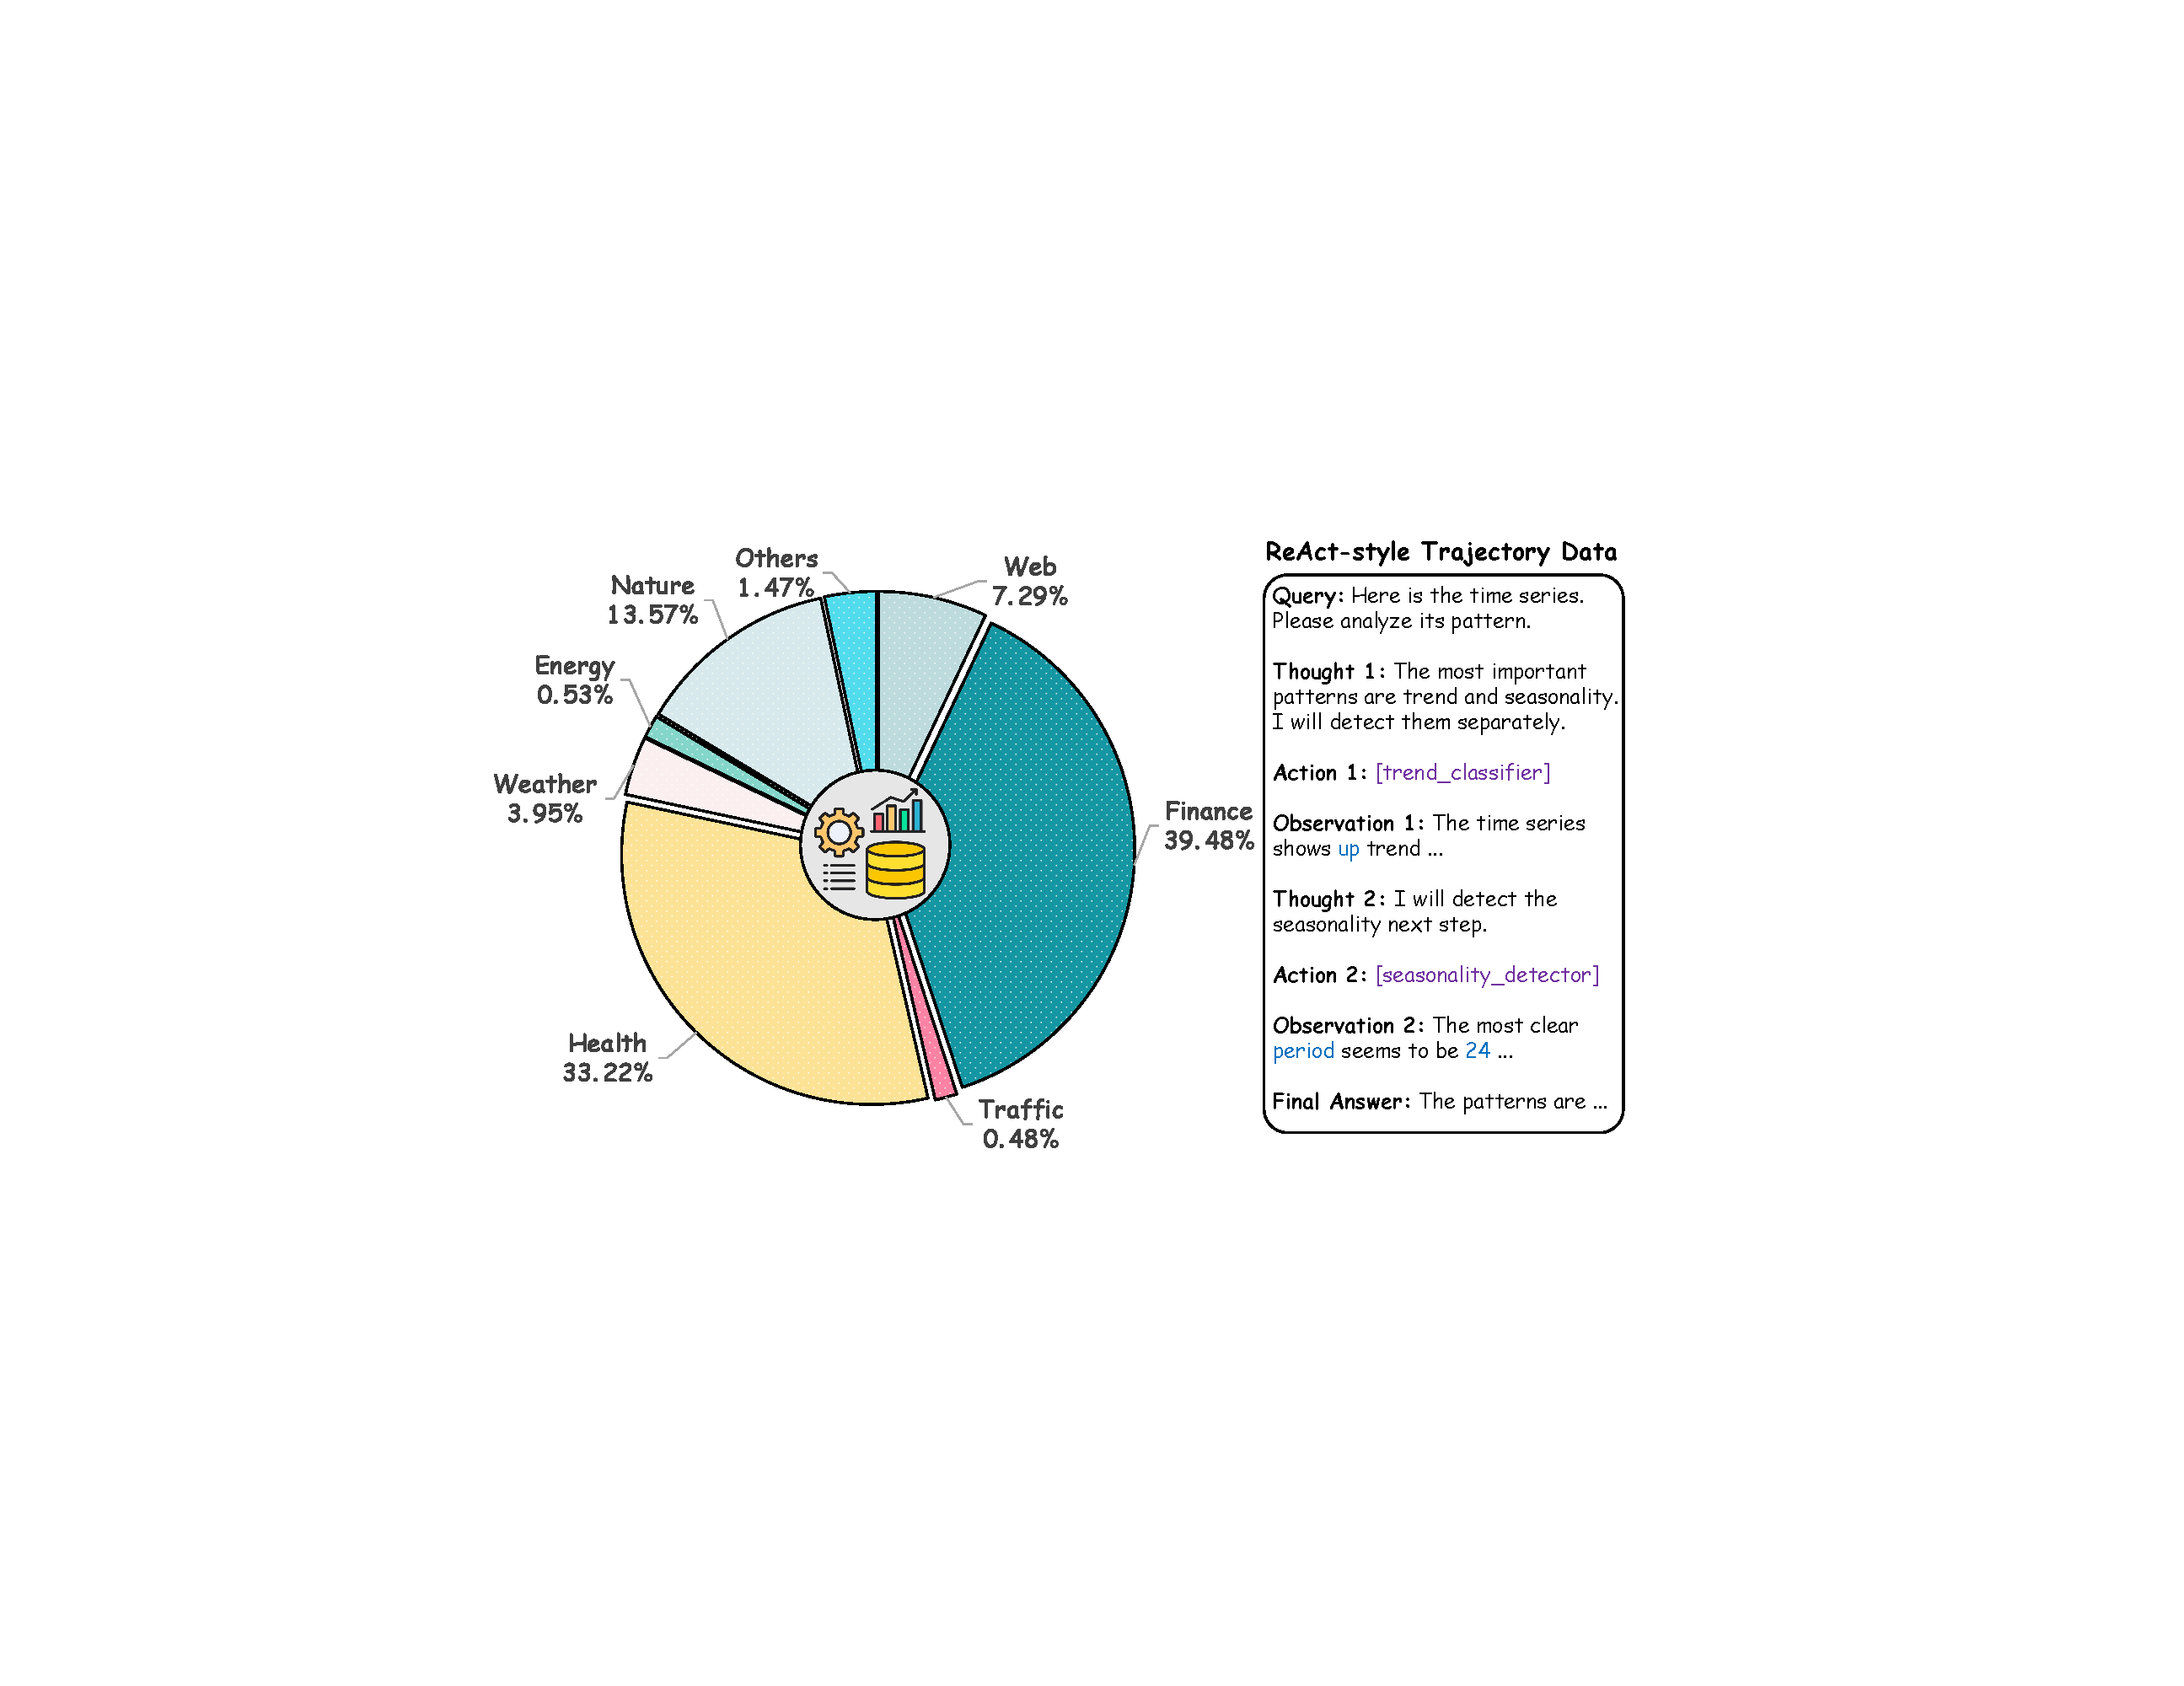
\includegraphics[width=1\linewidth]{Figures/dataset.pdf}
    \caption{Ratios of data sources in TimeToolBench (100k), the ReAct-style training corpus for agentic time series reasoning.}
\label{fig: dataset}
\end{figure}
With the help of TimeART, TSRMs can already utilize tools for reasoning. However, they still fall short in understanding the boundaries of tools' capabilities, which may cause suboptimal and conservative invocations. Intuitively, letting a senior data scientist demonstrate the standard trajectories, and leveraging TSRMs to learn the underlying principles is a feasible method, which has been widely applied in many other domains~\citep{gou2023tora,yao2022react}. To ensure the scale of the corpus, their approach often adopts powerful closed-source LLMs, e.g., Gemini-2.5, GPT-4, to replace human experts.

We collect and curate \textit{TimeToolBench}, which comprises over 100k tool-use trajectories with GTP-4o as the expert model, as shown in Figure~\ref{fig: dataset}. Since the tool-use trajectories are LLM artifacts, the original TSQA datasets used to generate them are from research teams~\citep{TimeMQA,cai2024timeseriesexam,chen2025mtbench,xie2024chatts}, which are from real-world applications or generated synthetically through human check, covering multiple domains shown in Figure~\ref{fig: dataset}. Compared with traditional chain-of-thought reasoning, this paradigm is able to generate both verbal reasoning traces and actions in an interleaved manner~\citep{yao2022react}. This enables LLMs to conduct dynamic reasoning to create, sustain, and adjust high-level action plans (reason to act). Simultaneously, it can interact with external environments to integrate supplementary information into the reasoning process (act to reason). Therefore, \textit{we also adopt the ReAct style in the inference phase of TimeART.}

During the collection of trajectories, we take some measures to ensure the quality of them--see Figure~\ref{fig: overview} (left). Given a TSQA sample $(\mathrm{Q}, y)$ with query $\mathrm{Q}$ and answer $y$, GPT-4o works like an expert and outputs a trajectory $\mathcal{T} := (\mathrm{Q}, (\mathrm{T}_1, \mathrm{A}_1, \mathrm{O}_1),\cdots,(\mathrm{T}_K, \mathrm{A}_K, \mathrm{O}_K), \mathrm{F})$. We first make coarse-grained answer check:
\begin{gather}
\text{Flag} = 
\begin{cases} 
1, & \text{with fixed options, } \mathrm{F} = y \\
1, & \text{open-ended, } \text{BERT-Score}(\mathrm{F}, y) > \sigma \\
0, & \text{otherwise}
\end{cases}
\end{gather}
For questions with fixed options, we ensure that the Final Answer F is completely consistent with y; for open-ended questions, since the answers are not fixed, we ensure that their semantic alignment with BERT-Score~\citep{reimers2019sentence} higher than a threshold $\sigma$. Then we filter out the trajectories with $\text{Flag}=0$. 
\begin{figure*}[!htbp]
    \centering

\includegraphics[width=1\linewidth]{Figures/overview.pdf}
    \caption{The overviews of the data pipeline for TimeToolBench (left), and the training pipeline for TimeART (right).}
\label{fig: overview}
\end{figure*}
To preserve the quality of the reasoning process, we further verify the intermediate logical chains. Among tuples $(\mathrm{T}_k, \mathrm{A}_k, \mathrm{O}_k)$, the reasoning behaviors mainly occur at $\mathrm{T}_k \rightarrow \mathrm{A}_k$ and $\mathrm{O}_{k-1} \rightarrow \mathrm{T}_k$. Therefore, we randomly sample subsequences from the trajectory $\mathcal{T}$ like $(\mathrm{O}_{k-1}, \mathrm{T}_k, \mathrm{A}_k )$. To evaluate their qualities, we use several strong LLMs~\citep{liu2024deepseek,achiam2023gpt,yang2025qwen3} as judgers. For each LLM judger, we randomly sample a logical chain $(\mathrm{O}_{k-1}, \mathrm{T}_k, \mathrm{A}_k )$ from the trajectory $\mathcal{T}$, prompt it to evaluate whether the logical chain is reasonable. Supposed that there exists $M$ LLMs, the quality evaluation process can be formulated as:
\begin{gather}
\text{Flag} = \bigwedge_{m=1}^M \text{LLM}^m(\mathrm{O}_{k_m-1}, \mathrm{T}_{k_m}, \mathrm{A}_{k_m}),
\end{gather}
where $\text{LLM}^m(\mathrm{O}_{k_m-1}, \mathrm{T}_{k_m}, \mathrm{A}_{k_m})=1$ denotes that the $m$-th LLM gives positive evaluation to the logical chain $(\mathrm{O}_{k_m-1}, \mathrm{T}_{k_m}, \mathrm{A}_{k_m})$. Only if all LLMs give positive evaluations to the logical chains assigned to them, the $\text{Flag}=1$ and the trajectory is saved. This method can keep the diversity through using different LLMs and evaluated parts~\citep{badshah2025reference}, and keep strictness through requiring unanimous approval. 


\subsection{Training strategy}
\label{sec: training strategy}
To avoid the common dilemmas in behaviour cloning and reinforcement learning, we devise a training strategy to encourage TSRMs to learn from early experience and self-reflection. This strategy consists of four stages, covering the underlying principles of conventional behaviour cloning and reinforcement learning, and providing a more direct manner to teach TSRMs strategic tool-use. 

\textbf{Stage 1: Teach TSRMs the capability boundary of tools.} Though the introductions of tools are organized as external constrains $\mathrm{E}$ to guide the invocations of TSRMs, they may not understand the actual capability of each tool. Under these circumstances, directly training TSRMs on TimeToolBench with behaviour cloning may lead to rigid imitation, thus hindering generalization. To tackle this problem, we first construct early experiences $\mathcal{D}_{exp}$ based on the collected trajectories. As shown in Figure~\ref{fig: overview} (right), considering a trajectory $\mathcal{T} := (\mathrm{Q}, (\mathrm{T}_1, \mathrm{A}_1, \mathrm{O}_1),\cdots,(\mathrm{T}_K, \mathrm{A}_K, \mathrm{O}_K), \mathrm{F})$ in TimeToolBench, we sample $J$ alternative tools for each Thought state $\mathrm{T}_k$ from the initial policy of the TSRM $p_\theta$: $\{\mathrm{A}_k^1, \cdots, \mathrm{A}_k^J\}$, then they lead to early experiences $\mathcal{D}_{exp}$: $\{(\mathrm{T}_k, \mathrm{A}_k^j, \mathrm{O}_k^j | \mathrm{S}_{1:3k-2})\}_{j=1,k=1}^{J,K}$, where $\mathrm{S}_{1:3k-2}$ are all previous states before $\mathrm{T}_k$. Then we train the TSRM $p_\theta$ to understand the capability boundary of tools:
\begin{gather}
    \mathcal{L}_1 = -\displaystyle\sum_{(\mathrm{T}_k, \mathrm{A}_k^j, \mathrm{O}_k^j | \mathrm{S}_{1:3k-2})}  \log p_\theta (\mathrm{O}_k^j | \mathrm{T}_k, \mathrm{A}_k^j, \mathrm{S}_{1:3k-2})
\end{gather}
This training objective allows TSRM $p_\theta$ to understand the transition rules with tool-use, and potential invalid and improper invocation experiences. Actually, it implicitly models a world model~\citep{gu2024your} by predicting the performance of tools in specific scenarios for agentic reasoning, which coarsely internalizes the dynamics into the TSRM.

\textbf{Stage 2: Teach TSRMs the strategies of tool-use.} After training the TSRM $p_\theta$ with objective $\mathcal{L}_1$, it can fully understand the functions of tools. In other words, Stage 1 serves as a good warmup phase, teaching the TSRM the basic use principles of TimeART. We then train TSRM for strategic tool-use:
\begin{gather}
    \mathcal{L}_2 = -\displaystyle\sum_{(\mathrm{T}_k,\mathrm{A}_k | \mathrm{S}_{1:3k-2})} \log p_\theta (\mathrm{A}_k | \mathrm{T}_k, \mathrm{S}_{1:3k-2})
\end{gather}
Note that though $\mathcal{L}_2$ is the conventional behaviour cloning objective, it guides the TSRM to learn from the expert model after the warmup of Stage 1, which may mitigate the overfitting phenomena.

\textbf{Stage 3: Build self-reflection samples to guide TSRMs.} Then we build a self-reflection process to guide the TSRM to learn from its own exploratory outcomes. Specifically, we first use the trained TSRM $p_\theta$ to summarize the underlying explanations for tool invocation, which can provide richer, transferable supervision than expert actions alone. The process can be formulated as:
\begin{gather} 
    \text{For }(\mathrm{T}_k, \mathrm{A}_k^j, \mathrm{O}_k^j) \text{ and } (\mathrm{T}_k, \mathrm{A}_k, \mathrm{O}_k),\\
    \mathrm{C}_k^j = p_\theta(\text{Why }\mathrm{A}_k \text{ not } \mathrm{A}^j_k \text{ ?}),
\end{gather}
where $\mathrm{C}_k^j$ is the summarized explanation, explaining why the expert action $\mathrm{A}_k$ is preferable to the alternative action $\mathrm{A}_k^j$ based on the differences between their resulting observations $\mathrm{O}_k$ and $\mathrm{O}_k^j$. Thus the self-reflection dataset $\mathcal{D}_{ref} = \{(\mathrm{T}_k, \mathrm{A}_k^j, \mathrm{C}_k^j | \mathrm{S}_{1:3k-2})\}_{j=1,k=1}^{J,K}$ can be obtained. Note that the concrete prompt used to generate the self-reflection explanations are listed in Appendix~\ref{app: prompt}. 

\textbf{Stage 4: Teach TSRMs to use which tools and the reasons.} We then train the TSRM $p_\theta$ to jointly predict the explanation $\mathrm{C}^j_k$ and the expert action $\mathrm{A}_k$ conditioned on the current state:
\begin{gather}
    \mathcal{L}_3 = -\displaystyle\sum_{(\mathrm{T}_k, \mathrm{A}_k^j, \mathrm{C}_k^j | \mathrm{S}_{1:3k-2})} \log p_\theta(\mathrm{C}^j_k, \mathrm{A}_k, | \mathrm{T}_k, \mathrm{S}_{1:3k-2})
\end{gather}
Intuitively, this process teaches the TSRM to invoke proper tools based on the summarized criteria. It is somewhat similar to reinforcement learning with reward functions, but more controllable without online rollouts and training imbalance problems. In practice, we mix the self-reflection dataset $\mathcal{D}_{ref}$ with the expert trajectories in  TimeToolBench to construct the training samples for $\mathcal{L}_3$.

To sum up, learning from the Stage 1 -- 4 encourages TSRMs to move beyond simple imitations of expert trajectories. These stages construct an alternative way to mitigate the common dilemmas of conventional behaviour cloning and reinforcement learning in agentic time series reasoning, which teach TSRMs to master the strategic tool-use and understand the underlying principles, thus developing more generalizable decision criteria.